\section{Random Triangles in High Dimensions}

For a triangle $\Delta$, we will let $\mathcal{Q}$ be a measure of the \textit{quality} of the triangle as defined by
\begin{equation}
\label{eq:triangle_score}
\mathcal{Q}(\Delta) = \frac{4\sqrt{3} A}{ \ell_1^2 + \ell_2^2 + \ell_3^2}
\end{equation}
where $A$ is the area of the triangle, and $\ell_1$, $\ell_2$ and $\ell_3$ are the lengths of the three sides.
Without performing any computations, can you determine the maximum and minimum values that $\mathcal{Q}$ can take? Can you describe what kinds of triangles are associated with high, and with low, values of $\mathcal{Q}$?

In the first part of this project, you will write a function that computes the quality of a triangle in $\mathbb{R}^2$, given the coordinates of its vertices.

\begin{itemize}
  \item Write a function, \texttt{tri\_lengths()}, that takes as its arguments the three vertices of a triangle and returns the lengths of the three sides of the triangle.  
  \item Write a function, \texttt{tri\_angles()}, that takes as its arguments the three vertices of a triangle and returns the angles of the triangle.
  \item Write a function, \texttt{tri\_area()}, that takes as its arguments the three vertices of a triangle and returns the area of the triangle.
  \item Write a function, \texttt{tri\_score()}, that takes as its arguments the three vertices of a triangle and returns the quality score of the triangle as defined in equation (\ref{eq:triangle_score}). 
  \item Test your function \texttt{tri\_score()} on the four triangles below. As a check on your function, the correct values are:
\begin{align*}
	\mathcal{Q}({\color{green}{\Delta}}) &= 0.597\cdots,
&	\mathcal{Q}({ \color{blue}{\Delta}}) &= 0.413\cdots,\\
	\mathcal{Q}({\color{red}{\Delta}}) &=0.172\cdots , 
&	\mathcal{Q}({ \color{purple}{\Delta}}) &= 1.
\end{align*}
\end{itemize}

\begin{center}
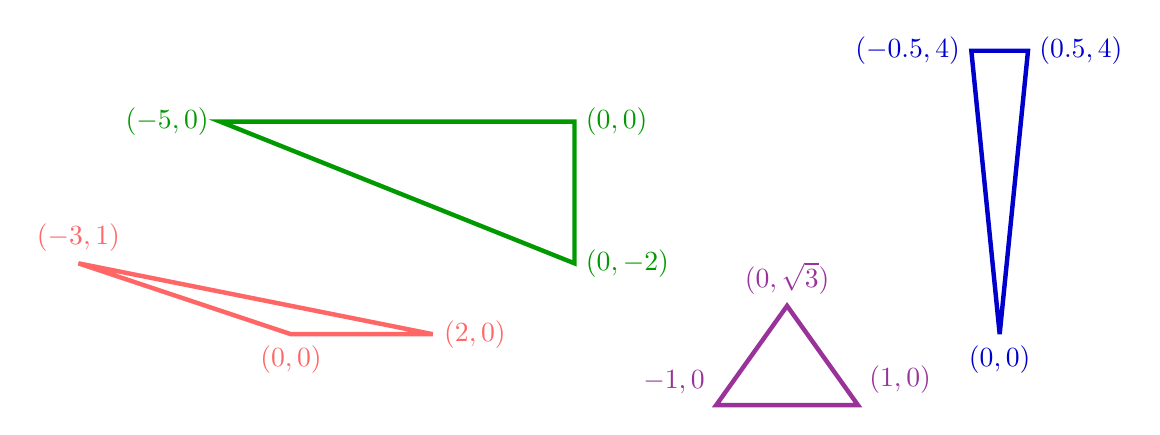
\begin{tikzpicture}[scale = 1.8]
  \draw[ultra thick,red!60!white] (0,0)node[below] {$(0,0)$} -- (-1.5,.5)node[above]{$(-3,1)$} -- (1,0)node[right]{$(2,0)$} --cycle;
  \draw[ultra thick, green!60!black] (-0.5,1.5)node[left] {$(-5,0)$} -- (2,1.5)node[right]{$(0,0)$} -- (2,.5)node[right]{$(0,-2)$} -- cycle;
  \draw[ultra thick, red!50!blue!80] (3,-.5)node[above left] {$-1,0$} -- (4,-.5)node[above right] {$(1,0)$} -- (3.5,.2)node[above]{$(0,\sqrt{3})$} -- cycle;
  \draw[ultra thick, blue!80!black] (5,0)node[below]{$(0,0)$} -- (4.8,2)node[left]{$(-0.5,4)$} -- (5.2,2)node[right]{$(0.5,4)$} -- cycle;
\end{tikzpicture}
\end{center}

Many applied mathematicians regularly work with data sets where each data point is associated with many different features (e.g. each medical patient is associated with their own temperature, heart rate, blood pressure, etc). 
Sometimes the physical, three-dimensional world can provide useful intuition for the geometry of higher dimensional space. Most of the time, however, we are unable to grasp all the weird ways that the higher dimensional space is `bigger'. 

In the second part of this project, you will compare the expected quality of random triangles in $\mathbb{R}^2$ with that of random triangles in $\mathbb{R}^{10}$.
\begin{enumerate}[(a)]
  \item 
  \begin{enumerate}[i.]
    \item Use a random number generator to create a random point, \(\bm{x} = (x_1,x_2)\), that is normally distributed in $\mathbb{R}^2$. The functions \texttt{randn()} (Matlab), \texttt{np.random.randn()} (Python), or \texttt{randn()} (Julia) may be useful.
    \item Repeat part i. until you have three points, $\bm{x} = (x_1,x_2)$, \(\bm{y} = (y_1,y_2)\), and \(\bm{z} = (z_1,z_2)\). Let $\Delta$ be the triangle with $\bm{x}$, $\bm{y}$, and $\bm{z}$ as its vertices. Use your function \texttt{tri\_score()} to compute $\mathcal{Q}(\Delta)$.
    \item Repeat parts i. and ii. until you have the quality scores for 100,000 random triangles. Plot a histogram of your data.
  \end{enumerate}
  \item Repeat this process for triangles in $\mathbb{R}^{10}$. That is, use a multivariate normal random number generator to generate 3 points in $\mathbb{R}^{10}$, $\bm{x} = (x_1,x_2,\dots x_{10})$, $\bm{y} = (y_1,y_2,\dots,y_{10})$, $\bm{z} = (z_1,z_2, \dots, z_{10})$. Let $\Delta$ be the triangle with $\bm{x}$, $\bm{y}$, and $\bm{z}$ as its vertices, and compute $\mathcal{Q}(\Delta)$. Repeat for 100,000 random triangles.
 \item Compare the histogram for triangles in $\mathbb{R}^2$ with a histogram for triangles in $\mathbb{R}^{10}$.  Provide a geometric explanation for why the random triangles in higher dimensions are much closer to equilateral than the random triangles in lower dimensions
\end{enumerate}
